\documentclass[11pt,a4paper,twoside,openright]{report}

\usepackage[top=25mm,bottom=25mm,right=25mm,left=30mm,head=12.5mm,foot=12.5mm]{geometry}
\let\openright=\cleardoublepage

\usepackage[a-2u]{pdfx}

\usepackage[
   backend=biber
%  ,style=iso-authoryear
  ,style=numeric%alphabetic
  ,citestyle=numeric
  ,sortlocale=en_US
  ,bibencoding=UTF8
  %,block=ragged
]{biblatex}
\addbibresource{references.bib}

%% Přepneme na českou sazbu, fonty Latin Modern a kódování češtiny
\usepackage[english]{babel}
\usepackage{lmodern}
\usepackage[T1]{fontenc}
\usepackage{textcomp}
\usepackage[utf8]{inputenc}

% Set fonts
%\RequirePackage[osf]{mathpazo} % Palatino with oldstyle figures
%\newcommand\liningnums[1]{\fontfamily{ppl}\selectfont#1}
%\RequirePackage{eulervm}
%\RequirePackage[scaled=.8819]{sourcecodepro} % Source Code Pro typeface for monospace

%%% Další užitečné balíčky (jsou součástí běžných distribucí LaTeXu)
\usepackage{amsmath}        % rozšíření pro sazbu matematiky
\usepackage{amsfonts}       % matematické fonty
\usepackage{amsthm}         % sazba vět, definic apod.
\usepackage{bm}             % tučné symboly (příkaz \bm)
\usepackage{graphicx}       % vkládání obrázků
\usepackage{fancyvrb}       % vylepšené prostředí pro strojové písmo
\usepackage{fancyhdr}       % prostředí pohodlnější nastavení hlavy a paty stránek
\usepackage{icomma}         % inteligetní čárka v matematickém módu
\usepackage{dcolumn}        % lepší zarovnání sloupců v tabulkách
\usepackage{booktabs}       % lepší vodorovné linky v tabulkách
\makeatletter
\@ifpackageloaded{xcolor}{
   \@ifpackagewith{xcolor}{usenames}{}{\PassOptionsToPackage{usenames}{xcolor}}
  }{\usepackage[usenames]{xcolor}} % barevná sazba
\makeatother
\usepackage{multicol}       % práce s více sloupci na stránce
\usepackage{caption}
\usepackage{enumitem}
\usepackage{lipsum}
\setlist[itemize]{noitemsep, topsep=0pt, partopsep=0pt}
\setlist[enumerate]{noitemsep, topsep=0pt, partopsep=0pt}
\setlist[description]{noitemsep, topsep=0pt, partopsep=0pt}
\usepackage{pdfpages}

\usepackage{tocloft}
\setlength\cftparskip{0pt}
\setlength\cftbeforechapskip{1.5ex}
\setlength\cftfigindent{0pt}
\setlength\cfttabindent{0pt}
\setlength\cftbeforeloftitleskip{0pt}
\setlength\cftbeforelottitleskip{0pt}
\setlength\cftbeforetoctitleskip{0pt}
\renewcommand{\cftlottitlefont}{\Huge\bfseries}
\renewcommand{\cftloftitlefont}{\Huge\bfseries}
\renewcommand{\cfttoctitlefont}{\Huge\bfseries}

% vyznaceni odstavcu
\parindent=0pt
\parskip=11pt

% zakaz vdov a sirotku - jednoradkovych pocatku ci koncu odstavcu na prechodu mezi strankami
\clubpenalty=1000
\widowpenalty=1000
\displaywidowpenalty=1000

% nastaveni radkovani
\renewcommand{\baselinestretch}{1.20}

% nastavení hlavy a paty stránek
\fancyhf{}
\renewcommand{\chaptermark}[1]{\markboth{#1}{}}
\fancyhead[RO,LE]{\leftmark}
\fancyfoot[RO,LE]{\thepage}
%\renewcommand{\footrulewidth}{0pt}
\fancypagestyle{plain}{%
\fancyhf{} % clear all header and footer fields
\fancyfoot[RO,LE]{\thepage}
\renewcommand{\headrulewidth}{0pt}
%\renewcommand{\footrulewidth}{0.5pt}
}

% Tato makra přesvědčují mírně ošklivým trikem LaTeX, aby hlavičky kapitol
% sázel příčetněji a nevynechával nad nimi spoustu místa. Směle ignorujte.
\makeatletter
\def\@makechapterhead#1{
  {\parindent \z@ \raggedright 
   \Huge\bfseries \thechapter. #1
   \par\nobreak
   \vskip 20\p@
}}
\def\@makeschapterhead#1{
  {\parindent \z@ \raggedright 
   \Huge\bfseries #1
   \par\nobreak
   \vskip 20\p@
}}
\makeatother

% Trochu volnější nastavení dělení slov, než je default.
\lefthyphenmin=2
\righthyphenmin=2

% Zapne černé "slimáky" na koncích řádků, které přetekly, abychom si
% jich lépe všimli.
\overfullrule=1mm

%% Balíček hyperref, kterým jdou vyrábět klikací odkazy v PDF,
%% ale hlavně ho používáme k uložení metadat do PDF (včetně obsahu).
%% Většinu nastavítek přednastaví balíček pdfx.
\hypersetup{unicode}
\hypersetup{breaklinks=true}
\hypersetup{hidelinks}

%%% Prostředí pro sazbu kódu, případně vstupu/výstupu počítačových
%%% programů. (Vyžaduje balíček fancyvrb -- fancy verbatim.)

\DefineVerbatimEnvironment{code}{Verbatim}{fontsize=\small, frame=single}

% \coloneqq and other symbols
\usepackage{mathtools}

% name of the project
\newcommand\pname{brandy0}

\newcommand\this{project}
\newcommand\software{software}
\newcommand\vxlisp{\vspace*{12pt}}
\newcommand\icd[1]{\texttt{#1}}
\newcommand{\ccd}[1]{\colorbox{gray!15!white}{\texttt{#1}}}
\newcommand{\scd}[1]{
	\vspace*{5pt}

	\ccd{#1}
	\vspace*{5pt}
}
\newcommand{\nscd}[1]{\scd{\$ #1}}
\newcommand{\sscd}[1]{\scd{\$ sudo #1}}
\newcommand{\aptinstall}[1]{\sscd{apt install #1}}
\newcommand{\snapinstall}[1]{\sscd{snap install #1}}
\newcommand{\defos}{Ubuntu 20.10}
\newcommand{\psubinst}{possible installation using \icd{snap} on \defos}
\newcommand{\pubinst}{possible installation using \icd{apt} on \defos}

\newcommand\dt{\Delta t}
\newcommand\dx{\Delta x}
\newcommand\dy{\Delta y}

%\newcommand\vxpder[2]{\frac{\partial #1}{\partial #2}}


\def\NazevPrace{Fluid Flow Simulator}
\def\Trida{R8.A}
\def\AutorPrace{Viktor Fukala}
\def\DatumOdevzdani{2021}

% Vedoucí práce: Jméno a příjmení
\def\Vedouci{Šimon Schierreich}

% Studijní program a obor
%\def\StudijniProgram{studijní program}
%\def\StudijniObor{studijní obor}

% Text čestného prohlášení
%\def\Prohlaseni{Prohlašuji, že jsem svou práci vypracoval samostatně a použil jsem pouze prameny a literaturu
%uvedené v~seznamu bibliografických záznamů. Nemám žádné námitky proti zpřístupňování této práce v~souladu se
%zákonem č. 121/2000 Sb. o~právu autorském, o~právech souvisejících s~právem autorským a
%o~změně některých zákonů (autorský zákon) ve znění pozdějších předpisů.}
\def\Prohlaseni{I hereby declare that I created this \this{} unaidedly and that all sources I used are listed in the attached bibliography. I consent to this \this{} being made available in accordance with the Czech copyright law, Law No.\ 121/2000 (\emph{zákon č.\ 121/2000 Sb.\ o~právu autorském, o~právech souvisejících s~právem autorským a o~změně některých zákonů (autorský zákon)} in Czech).}

% Text poděkování
\def\Podekovani{%
	The creation of this project in its ultimate form would not be possible without the help, support, and advice from my supervisor, Šimon Schierreich. I would like to thank him for supervising this \this{} and always being ready to answer my questions and clear my doubts.
}

% Abstrakt česky
\def\Abstrakt{%
	Software vyvinutý v rámci této práce je nativní aplikací pro operační systémy Linux a Windows, která simuluje a vizualizuje proudění nestlačitelné tekutiny kolem libovolných pevných překážek ve dvourozměrném prostoru za různých podmínek. Jeho cílem je prohloubit základní povědomí o~proudění tekutin u koncových uživatelů pomocí fyzikálně přesných vizualizací bez nutnosti ovládat složitá rozhraní, jež bývají součástí průmyslového software pro simulaci tekutin. Proudění tekutiny se simuluje na základě tvarů překážek a okrajových podmínek pro tlak a pro rychlost, což koncový uživatel zadává před spuštěním simulace. Nejrychleji a nejspolehlivěji náš software pracuje při nízkých Reynoldsových číslech (laminární proudění), zatímco při vysokých Reynoldsových číslech (turbulentní proudění) začíná potřebný výpočetní výkon prudce narůstat. I přesto náš software dosahuje svého cíle tím, že je schopen simulovat širokou škálu laminárních proudění a jevů při přechodu k turbulentnímu proudění (např.\ vznik vírů).
}

% Abstrakt anglicky
\def\AbstraktEN{%
The \software{} developed in this \this{}, \pname{}, is a native application for Linux and Windows that simulates and visualizes the flow of an incompressible fluid around arbitrary solid obstacles and under various conditions in two-dimensional space. It aims to deepen the basic understanding of fluid flow among its end-users by presenting physically accurate visualizations without the sophisticated interface that often comes with fluid simulation software used in the industry. It simulates the flow based on the shapes of the obstacles and the boundary conditions for pressure and velocity, all of which can be configured by the end-user before starting the simulation. The \software{} works the fastest and most reliably for low Reynolds numbers (laminar flow), whereas for high Reynolds numbers (turbulent flow), the amount of required computational power (both in time and space) increases rapidly. Nevertheless, the \software{} achieves its goal by being able to simulate a wide range of laminar flows and phenomena (such as the development of vortices) during at the transition to turbulent flows.
}

% 3 až 5 klíčových slov
\def\KlicovaSlova{výpočetní dynamika tekutin, Navier-Stokesovy rovnice pro nestalčitelné tekutiny, vizualizace dat, počítačové simulace}
% 3 až 5 klíčových slov anglicky
\def\KlicovaSlovaEN{computational fluid dynamics, incompressible Navier-Stokes equations, data visualization, computer simulation}


\begin{document}

%%% Titulní strana práce a další povinné informační strany

%%% Titulní strana práce

\pagestyle{empty}
\pagenumbering{gobble}
\hypersetup{pageanchor=false}

\begin{center}
\LARGE
\textbf{GYMNASIUM JANA KEPLERA}\\
{\large Parléřova 2/118, 169 00 Praha 6}

\vspace{\stretch{3}}

\includegraphics[width=.3\textwidth]{img/logo}

\vspace{\stretch{3}}

{\Huge\bfseries\NazevPrace}

\vspace{8mm}
\mdseries{Maturita Project}

\vspace{\stretch{8}}
\large
\begin{tabular}{rl}
Author: & \AutorPrace \\
\noalign{\vspace{2mm}}
Class: & \Trida\\
\noalign{\vspace{2mm}}
School year: & 2020/2021\\
\noalign{\vspace{2mm}}
Subject: & Computer Science \\
\noalign{\vspace{2mm}}
Supervisor: & \Vedouci \\
\end{tabular}

\vspace{20mm}
Prague, \DatumOdevzdani
\end{center}


\openright

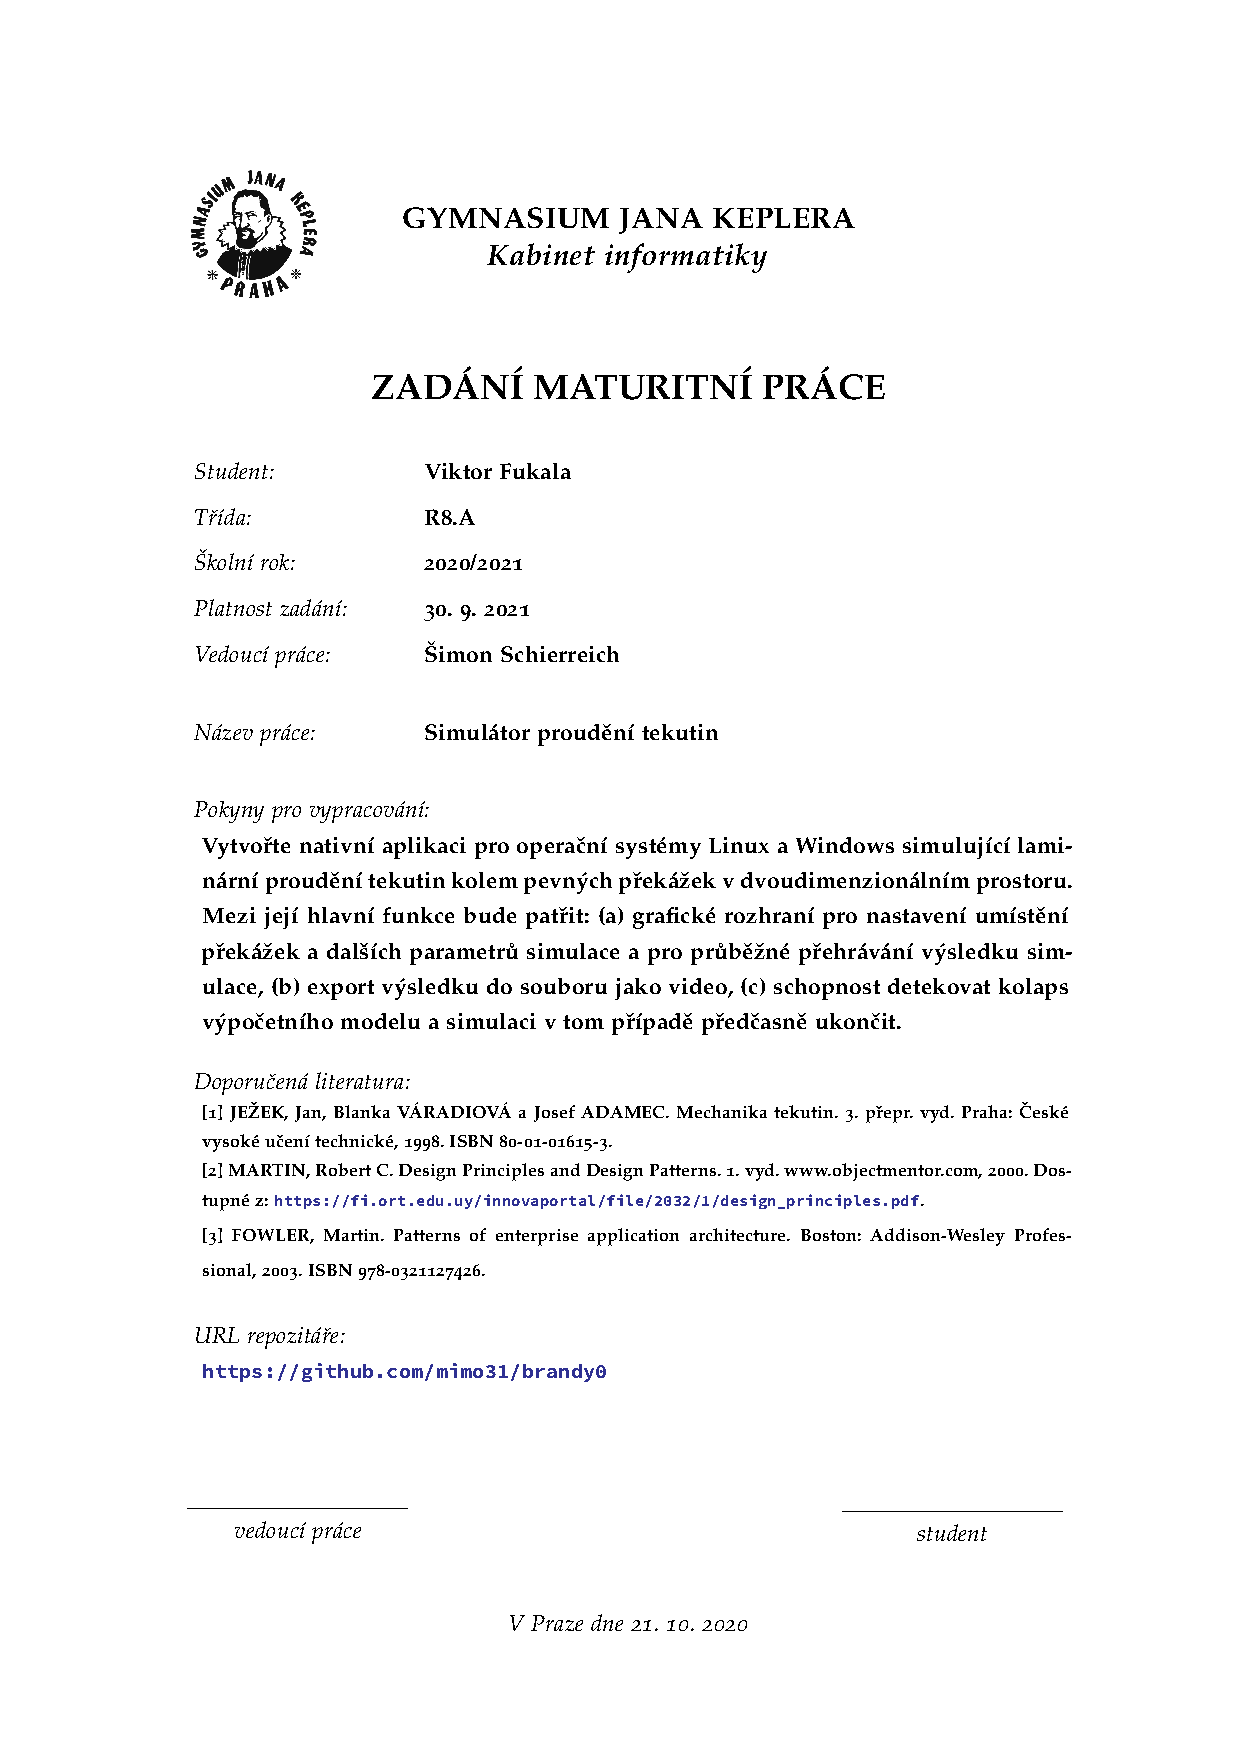
\includepdf[]{zadani.pdf}


%%% Strana s čestným prohlášením k bakalářské práci

\hypersetup{pageanchor=true}
\cleardoublepage
\vspace*{\fill}
\section*{Declaration of Authorship}
\noindent
\Prohlaseni

\vspace{2cm}
\noindent
Prague, \today
\hspace*{\fill}\small{\AutorPrace}
\vspace{1cm}

%%% Poděkování
\openright
\vspace*{\fill}
\section*{Acknowledgements}
\noindent
\Podekovani
\vspace{1cm}


%%% Povinná informační strana bakalářské práce
\openright
\section*{Abstrakt}
\noindent
\Abstrakt
\subsection*{Klíčová slova}
\noindent
\KlicovaSlova

\bigskip\bigskip\bigskip
\section*{Abstract}
\noindent
\AbstraktEN
\subsection*{Keywords}
\noindent
\KlicovaSlovaEN

\openright
\pagenumbering{arabic}


% Obsah
\setcounter{tocdepth}{2}
\tableofcontents

\chapter{Theoretical Background}
\pagestyle{fancy}

\section{Introduction}
Computational fluid dynamics (CFD) is the application of numerical methods to fluid flow problems. As of today, it plays a vital role in engineering areas and the related industries such as aeronautics, the automotive industry, environmental engineering, bioengineering (simulating the blood flow or the air flow in lungs, for example), or even video games, where it is used to produce realistic video of fluids. Computer-simulated fluid flow has replaced many expensive or even technically infeasible real-world experiments, and its importance is only expected to grow with future advancements in both computing power and the efficiency of the applied algorithms.

In this \this{} however, we are not focused on any of these direct applications but rather on providing the end-user with the fundamental understanding of fluid flow phenomena and a high degree of freedom in experimenting -- i.e.\ setting up simulations to their liking. We aim to present \software{} that visualizes the computed results in an attractive and immediate manner, so that our goals differ greatly from those of the software used in the industry, as that often prioritizes precision and efficiency and comes with an elaborate user interface and special functionality for the one or the other engineering or industry application.

My main motivation for committing myself to the development of the \software{} constituting this \this{} was my fascination with the computers' ability to simulate (parts of) the real world and my curiosity as to how far one can get with only the general knowledge of physics and numerical analysis fundamentals and no prior expertise in CFD specifically.

Our \software{} computes and visualizes the temporal evolution of the state of a fluid inside a two-dimensional, rectangular container. The state of the fluid is given by the velocity vector field and the pressure scalar field, each of which has a value at every point inside the container. This state at some given time after the start of the simulation depends on a multitude of parameters:
\begin{itemize}
	\item \textbf{the shape of the container,}\\
		This includes the dimensions of the rectangular enclosing container and also the shapes and dimensions of the solid obstacles inside it. Both can be freely configured by the end-user before a simulation.
	\item \textbf{the mechanical properties of the fluid,}\\
		This includes the density and the viscosity of the fluid, of which both can be freely configured by the end-user.
	\item \textbf{the boundary conditions at the boundary of the container, and}\\
		At the four sides of the outer container, the user can specify what boundary conditions will be enforced. For both velocity and pressure, they can choose between a Dirichlet type or a Neumann type boundary condition. For the Dirichlet type boundary condition, they can also specify the value (of pressure or velocity) at the boundary. Under a Neumann type boundary condition we specifically understand a the Neumann boundary conditions which requires the derivative along the normal to the surface to be zero.
		\vxlisp

		At the inner boundaries, i.e.\ at the surface of the solid obstacles inside the container, the no-slip condition is enforced for velocity (meaning that a Dirichlet type boundary condition setting the velocity to the zero vector holds) and a Neumann type boundary conditions is set for pressure.
	\item \textbf{the initial conditions.}\\
		I.e.\ the state of the fluid at $t=0$. The state of the fluid at $t=0$ is set to zero velocity and zero pressure everywhere (except at the boundary).
\end{itemize}

\section{Physical Model}
To model the behavior of the fluid, we use the Navier-Stokes equations. Let $\mathbf u$ denote the velocity of the fluid and $p$ its pressure at all the points inside the container. We assume that the fluid is incompressible, so we get the incompressibility equation
\newcommand{\uu}{\mathbf u}
\newcommand{\D}{\mathrm D}
\begin{align}\label{eq:incom}
	\nabla\cdot\uu=0.
\end{align}
Then we have the Navier-Stokes momentum equation
\newcommand{\conv}{\frac{\D\uu}{\D t}}
\begin{align*}
	\rho\conv=-\nabla p+\mu\nabla^2\uu+\rho\mathbf g,
\end{align*}
where $\rho$ is the density of the fluid, $\mu$ its (dynamic) viscosity, $\mathbf g$ is the acceleration due to external forces (such as gravity) and $\conv$ denotes the material (also known as \emph{convective}) derivative of the velocity.
\newcommand{\pder}[2]{\frac{\partial #1}{\partial #2}}
\begin{align*}
	\conv=\pder\uu t+(\uu\cdot\nabla)\uu
\end{align*}
We assume no external forces, so $\mathbf g=0$. Hence, the momentum equation that we work with takes the form
\begin{align}\label{eq:momentum}
	\pder\uu t+(\uu\cdot\nabla)\uu=-\frac1\rho\nabla p+\nu\nabla^2\uu,
\end{align}
where $\nu=\mu/\rho$ is the \emph{kinematic} viscosity.
\section{Numerical Model}
Our way of numerically solving the above equations that is not the most accurate or computationally efficient, but it is relatively simple to implement and to work with. It is essentially the Chorin's projection method introduced in \cite{Chorin}. What I have implemented in an explicit, finite difference method.

% TODO resolve that Barba's materials are also mentioned in 2.2 Course of Development
During the implementation, Lorena A. Barba's practical examples of solving the Navier-Stokes equations \cite{CFDpython} as well the recordings of her CFD course at Boston University \cite{BarbaCourse} were of great help. The solver used in \cite{CFDpython} is an implementation of Chorin's projection method, and is therefore similar to our implementation, but there are also some notable differences such as the fact that the solver in \cite{CFDpython} neglects some of the terms on the right-hand side of the pressure Poisson equation, doesn't incorporate any obstacles inside the enclosing rectangular boundary, and doesn't use the general upwind differencing scheme as we do.

In order to computationally represent, process, and manipulate the state of the fluid, we must discretize in both space and time. As for the temporal discretization, we only compute the state of the fluid at times that are (non-negative) integer multiples of some small time $\dt$. These are computed successively with a state at any particular time depending on the state directly before. Each of the states must also be discretized spatially. For that, we use a uniform Cartesian grid with a spacing of $\dx$ and $\dy$ in the $x$ and the $y$ direction respectively and we store values of the fluid state fields only at these grid points.

\subsection{Temporal Discretization}
What now follows is a brief description of Chorin's projection method that we use in the core of our simulator.

Let us denote the value of a particular quantity at the $i$-th iteration by $i$ in the superscript. That is, let $\uu^i$ be the velocity field at the $i$-th iteration, $p^i$ the pressure field at the $i$-th iteration, $\left(\pder\uu t\right)^i$ the time derivative of the velocity field at the $i$-th iteration. Then we approximate the derivative of $\uu$ by the forward difference.
\begin{align*}
	\left(\pder{\uu}t\right)^i=\frac{\uu^{i+1}-\uu^i}{\dt}
\end{align*}
So at the $i$-th iteration, \eqref{eq:momentum} takes the form
\begin{align*}
	\frac{\uu^{i+1}-\uu^i}{\dt}+(\uu^i\cdot\nabla)\uu^i=-\frac1\rho\nabla p^i+\nu\nabla^2\uu^i.
\end{align*}
Together with the equation $\nabla\cdot\uu^{i+1}=0$ (that is \eqref{eq:incom} at the $(i+1)$-th iteration), this allows us to solve for $\uu^{i+1}$ and $p^i$. We express
\begin{align*}
	\uu^{i+1}=-\frac\dt\rho\nabla p^i+\dt\left(\nu\nabla^2\uu^i-(\uu^i\cdot\nabla)\uu^i\right)+\uu^i.
\end{align*}
\newcommand{\ww}{\mathbf w}
During the computation, we have yet to solve for $p^i$, so we only calculate the following intermediate vector field $\ww^i$.
\begin{align*}
	\ww^i\coloneqq\dt\left(\nu\nabla^2\uu^i-(\uu^i\cdot\nabla)\uu^i\right)+\uu^i
\end{align*}
The above formula gives the value of the field in the interior of the grid and we use the boundary conditions for velocity to calculate its values at the boundary. Then
\begin{align*}
	-\frac\dt\rho\nabla p^i+\ww^i=\uu^{i+1}
\end{align*}
and
\begin{align*}
	-\frac\dt\rho\nabla^2p^i+\nabla\cdot\ww^i=\nabla\cdot\uu^{i+1}=0.
\end{align*}
Hence, we have the following Poisson equation for $p^i$
\begin{align*}
	\nabla^2p^i=\frac\rho\dt\nabla\cdot\ww^i.
\end{align*}
We solve this Poisson equation\footnote{There exist several well-known methods for solving a Poisson equation numerically. They include, most notably, the Jacobi method, the Gauss-Seidel method, successive over-relaxation, multigrid methods, and the conjugate gradient method. Multigrid methods and the conjugate gradient method generally converge faster, but are noticeably more complex and difficult to implement than the other approaches mentioned. Of those, we use successive over-relaxation by default as it tends to have the fastest convergence. See section 9.3.3 of \cite{Epperson} for more details about the methods.} for $p^i$ in the interior of our grid and apply the boundary conditions for pressure to obtain $p^i$ at the boundary.

At last, we compute $\uu^{i+1}$ given by
\begin{align*}
	\uu^{i+1}=-\frac\dt\rho\nabla p^i+\ww^i
\end{align*}
and the boundary conditions for velocity.

\subsection{Spacial Discretization}
It remains to clarify how we compute the space derivatives of the various fields. As mentioned above, we use the method of finite differences. In particular, for the Laplacian, we use the five-point stencil
\begin{align*}
	(\nabla^2\uu^i)_{j,k}&=\frac{\uu^i_{j+1,k}-2\uu^i_{j,k}+\uu^i_{j-1,k}}{(\dx)^2}+\frac{\uu^i_{j,k+1}-2\uu^i_{j,k}+\uu^i_{j,k-1}}{(\dy)^2}\\
	(\nabla^2p^i)_{j,k}&=\frac{p^i_{j+1,k}-2p^i_{j,k}+p^i_{j-1,k}}{(\dx)^2}+\frac{p^i_{j,k+1}-2p^i_{j,k}+p^i_{j,k-1}}{(\dy)^2},
\end{align*}
where ${}_{j,k}$ in the subscript denotes that the value of the field at the $j$-th grid point in the $x$ direction and the $k$-th in the $y$ direction. For gradient and the divergence, we use the central difference
\begin{align*}
	(\nabla\cdot\ww^i)_{j,k}&=\frac{(\ww^i_x)_{j+1,k}-(\ww^i_x)_{j-1,k}}{2\dx}+\frac{(\ww^i_y)_{j,k+1}-(\ww^i_y)_{j,k-1}}{2\dy}\\
	((\nabla p)_x)_{j,k}&=\frac{p_{j+1,k}-p_{j-1,k}}{2\dx}\\
	((\nabla p)_y)_{j,k}&=\frac{p_{j,k+1}-p_{j,k-1}}{2\dy},
\end{align*}
where ${}_x$ (or ${}_y$) in the subscript refers to the $x$ (or the $y$) component of a vector field.

The discretization of the advection term ($(\uu^i\cdot\nabla)\uu^i$) is slightly more involved. We use upwind differencing\footnote{For a more detailed discussion of upwind differencing and some more advanced (and accurate) methods with the same purpose (albeit in a more general setting), see chapter 3 of \cite{OsherFedkiw} or only section 3.2 for upwind differencing specifically.} to ensure that the information about the fluid velocity is properly passed in the direction of the flow. That means that we take
\begin{align}\label{eq:advx}
	(\uu^i_x)_{j,k}\left(\pder{\uu^i}{x}\right)_{j,k}=(\uu^i_x)_{j,k}\cdot\frac1\dx\cdot\begin{cases}
		\uu^i_{j,k}-\uu^i_{j,k-1} & \text{for }(\uu^i_x)_{j,k}>0\\
		\uu^i_{j,k+1}-\uu^i_{j,k} & \text{for }(\uu^i_x)_{j,k}<0
	\end{cases}
\end{align}
and
\begin{align}\label{eq:advy}
	(\uu^i_y)_{j,k}\left(\pder{\uu^i}{y}\right)_{j,k}=(\uu^i_y)_{j,k}\cdot\frac1\dy\cdot\begin{cases}
		\uu^i_{j,k}-\uu^i_{j-1,k} & \text{for }(\uu^i_y)_{j,k}>0\\
		\uu^i_{j+1,k}-\uu^i_{j,k} & \text{for }(\uu^i_y)_{j,k}<0
	\end{cases}.
\end{align}
By definition, the advection term is the sum of the terms in \eqref{eq:advx} and \eqref{eq:advy}.
\begin{align*}
	((\uu^i\cdot\nabla)\uu^i)_{j,k}=(\uu^i_x)_{j,k}\left(\pder{\uu^i}{x}\right)_{j,k}+(\uu^i_y)_{j,k}\left(\pder{\uu^i}{y}\right)_{j,k}
\end{align*}

\chapter{Implementation}

\section{Used Technologies}
\subsection{Base Programming Language: C++}
The \software{} is written mostly in C++\footnote{See \cite{cppreference} for a good C++ reference.}. C++ is a compiled programming language with multiple freely available compilers, which are capable of many optimizations, so that the resulting executable programs are one of the fastest when compared to other programming languages. This is important for us because computational resources (and their efficient use) are a limiting factor during the simulations. Moreover, C++ code can be written in a highly structured manner (e.g.\ using objects and classes, namespaces, templates, \icd{constexpr}, \icd{const}, static assertions, etc.), which decreases the likelihood of errors altogether or at least enables better static analysis and the discovery of potential errors at compile time (compared to the C programming language, for example). 

\subsection{User Interface, Widget Toolkit}
The most visible technology used in the \software{} is gtkmm 3 \footnote{The official tutorial can be found in \cite{gtkmm3} and the official reference manual in \cite{gtkmm3ref}.}, a C++ wrapper around GTK+ 3 \footnote{The official reference manual including some examples and an explanation of the GTK+ general principles is in \cite{gtk3ref}. When working with gtkmm, it is rarely useful -- only in the exceptional cases when the gtkmm reference is not comprehensive enough.} user interface widget toolkit library. It is one of the two most widely used user interface libraries for C++, the other being Qt\footnote{See \cite{qt}.}. Qt is written natively in C++ (in contrast to GTK being a C library), but the gtkmm wrapper for C++ makes good use of C++ paradigms, so that gtkmm interoperates with C++ code just as easily. Hence, both gtkmm and Qt seemed adequate for our \software{} and the final decision was based on a personal preference for the GNOME ecosystem.

\subsection{OpenGL for Visualizations}
Specifically for the visualization of the simulated fluid flow, we use the OpenGL API\footnote{Reference in \cite{openglref}.} to produce detailed images accurately representing the computed states easily and to do so fast enough to be able to play the images as a continuous video. No complex graphics was necessary for our \software{}, so only 4 relatively simple shaders written in the OpenGL Shading Language are a part of the source code.

\subsection{FFmpeg for Writing Video Files}
% TODO: add link
Since the \software{} was required to be able to produce video files with the visualized flow of the fluid, we used the FFmpeg libraries for video manipulation. See section \ref{sec:runtimedeps} for the exact information about the FFmpeg libraries\footnote{Documentation is to be found in \cite{ffmpegdoc}.} used. Even though these are C libraries and so their API violates the principles of good design in C++, we use them because they are one of the most widely used tools for this kind of tasks and we are able to keep the interaction with their C API local within our codebase.

\subsection{CMake for Build Automation}
Compiling a C++ project can quickly become a demanding task as the complexity of the project increases. It is due to long compile times and also the necessary configuration that has to be done by whoever is trying to compile the project. CMake\footnote{Documentation in \cite{cmakedoc}.} saves time in both of these by not rebuilding the entire project on each build and by allowing its user to define build targets and organize the project configuration into flexible CMake configuration files.

\section{Course of Development}
% TODO resolve that Barba's materials are already mention in 1.3 Numerical model
At the beginning (September 2020 -- November 2020), we searched for and tried multiple physical models (e.g.\ incompressible or compressible fluid) and numerical models (various computation schemes) and we researched other software that already solves problems similar to what we aimed to do. There certainly exist other similar programs such as Flowsquare\footnote{See \cite{Flowsquare}.} or OpenFOAM\footnote{See \cite{OpenFOAM}.}. Both of these are generally allow for more sophisticated simulations, but they also typically require configuration outside of the program's own interface (e.g.\ preparation of bitmaps file with solid obstacles (Flowsquare) or writing the complete simulation setup into a configuration file (OpenFOAM)). Our software tries to be more accessible for less technically skilled users.

% TODO: add citations, add image
For the sake of simplicity, we started to focus only on incompressible flow. Besides Wikipedia articles such as \cite{WikiNavierStokes}, \cite{WikiJacobi}, \cite{WikiGaussSeidel}, and \cite{WikiSOR}, the most useful source of practical information were Lorena A. Barba's materials on CFD (refer to \cite{CFDpython}) and the recordings of her CFD course at Boston University (see \cite{BarbaCourse}). Throughout these initial stages of the development, we needed to perform many experiments in order to determine how reliably our numerical models work. A sizeable portion of the models were unstable and resulted in the computation diverging [add image of a diverging simulation]. Generally, we can say that none of our models (including the final one) could efficiently simulate turbulence (flow with a high Reynolds number).

In December, the development continued with the implementation of the main parts of the simulation configuration interface and the OpenGL visualization. The interface for the configuration of solid obstacles was implemented mainly in January and in February, controls for the video playback and the option to export video were added. Throughout March, parts of the numerical model were improved (including its efficiency), more options for the configuration of boundary conditions were made possible and various minor parts of the \software{} were improved, expanded, or fixed.

% other ideas of what went well:
% * use of CMake (flexible, shorter (taking less time to compile), and easier (less configuration work) builds)
% * drawing data for video export -- just swapping buffers and then drawing as usual, but there is some ugliness to the passing of the GL context
\section{Elegant and Efficient Solutions during Development}
% TODO improve word choice
This section discusses a few parts of the project that could be regarded as well tackled [<- word choice perhaps too informal] or as problems elegantly solved.

\subsection{Obstacle Configuration Interface}
One could argue that the obstacle configuration interface is, in contrast to other components of the \software{}, elegant and user-friendly. It displays to the user the obstacle they are about to add and the grid points that will become solid as a result of that, it allows them to sequentially undo and redo the addition of obstacle, or it allows to cancel the addition of a new obstacle. However, this might be, in part, caused by the relative isolation and clearly defined bound of this interface is supposed to do in the first place, particularly when the rest, the majority, and the core of the \software{} is rather volatile.

Nevertheless, there is room for improvement even in this interface. For example, the performance (and thus the smoothness of the UI) worsens as the number of points grows large enough and the editor lacks any ability to copy or move the added obstacles.

\subsection{Use of C++ Paradigms}
It is highly debatable claim to say that in general, the structure of the codebase is well design. But let us draw the attention to at least some specific part of the code that one may regard as well-design.

Firstly, notice the structs defined in the \icd{lib} directory -- namely \icd{Grid}, \icd{vec2d}, \icd{Point}. The \icd{Grid} struct is a generic two-dimensional container of fixed size and is used to represent the values of a quantity at the grid points inside a container. The \icd{vec2d} struct is a representation of a two-dimensional vector (with two coordinates of type \icd{double}) and \icd{Point} of a point with two integer coordinates. All these structs make heavy use of operator overloading, so that they can be used more easily and naturally. That includes a natural way of addressing the data in a \icd{Grid}, so that statements like
\begin{align*}
	\icd{g(3, 4) = g(0, 1)}
\end{align*}
or even
\begin{align*}
	\icd{g(p1) = g(p0)},
\end{align*}
where \icd g is of type \icd{Grid<T>} for any type \icd{T} that is copy assignable and $\icd{p0}$, $\icd{p1}$ are of type $\icd{Point}$, can be used (provided that the specified indices or points are within the bounds of the grid). Naturally, standard vector operation are also available through overloaded operators, so
\begin{align*}
	&\icd{p = (u.dot(a) / u.dot(u)) * u}\\
	&\icd{d = (a + b) / 2 + c * 1.5}
\end{align*}
are valid statements for \icd a, \icd b, \icd c, \icd d, \icd p, \icd u of type \icd{vec2d}.

On a similar note, we implemented a generic class \icd{Hideable} (in \icd{hideable.hpp}), which allows us to hide a GTK widget while it still takes up space in its parent container. The elegance of this generic class is that \icd{Hideable<T>} inherits from \icd T, so that a widget of type \icd W can be declared as \icd{Hideable<W>} and all its methods and attributes are still accessible normally while it now also has the new methods that hide and show (unhide) it.

However, other parts of the codebase are not so well designed. For example, the classes representing the program's windows and the classes representing the various stages of configuring / running a simulation try to follow a general pattern, but mainly due to the large number of different states the user interface can be in, they contain a relatively high amount of loosely structured code.

\subsection{Buffering of Computed Frames}
When computing the frames of a simulation, our \software{} does not know how much time (how many frames) it will run for. The time for which the simulator runs is under the full control of the user, as they can pause or resume the computation at any time. Therefore, the \software{} needs a flexible container to store the computed frames.

The \software{} uses a specific method to tackle this problem. A method which is elegantly simple and scalable with the number of frames, but it definitely has drawbacks too. One of the parameters of a simulation is the maximum number of frames that can be stored at once. When the simulation starts, the newly computed frames are being stored until the set capacity is reached. When the capacity is reached, every other of the already stored frames gets deleted and after this moment, only every other frame is stored. This coarsening of the temporal resolution by a factor of two is repeated every time the capacity is reached.

This method prevents the consumption of too much memory and it ensures that frames representing the entire duration of the computed simulation are still available at a reasonable temporal resolution. It is also probably one of the simplest solutions to achieve this. Besides the overall capacity, it does not require any configuration from the user.

Nevertheless, this approach might be inadequate in some cases. It not unusual that at the beginning of a simulation, there is a short time of drastic changes in the state of the fluid. Then, if the simulator runs for long enough, the temporal resolution might degrade so much that only a few frames, if any, show what happened during that short initial period of time. It could therefore be of value to allow for a variable temporal resolution during the simulation (typically high at the beginning, lower as the simulation progresses). Such an approach would however be unlikely to reach its full potential unless the user were able to configure these changes in resolution.

\section{Technical Complications during Development}

\subsection{Segmentation Fault due to \icd{GtkSwitch}}

The \software{} contained a bug which sometimes lead to a segmentation fault during the closing of the program. Since this did not interfere with the \software{}'s functionality in any way, fixing the crash was not a priority until later in the development process. It then turned out that the crash occurs inside the destructor of gtkmm's \icd{Gtk::Switch}, which internally calls some methods of the GTK's \icd{GtkSwitch} (notice no scope resolution operator) widget.

At that time, there was already a report\footnote{See \cite{GtkmmSwitchReport}.} of an issue in gtkmm that demonstrated the crash on a much simpler example. After some debugging of the gtkmm and GTK libraries, we concluded that there was a bug in the underlying GTK library, which leads to a null pointer being dereferenced whenever the destruction method is called on a \icd{GtkSwitch} that is still a part of some window. This has been reported\footnote{See \cite{GtkSwitchReport}.} in the GTK issue tracker on March 5, 2021 and has not been fixed as of today. Note that this bug only affects GTK+ 3 and not the newer but incompatible GTK 4.

In our \software{} the crash can be avoided by removing the \icd{Gtk::Switch} from the window before the \icd{Switch} gets destroyed, which is exactly what the \software{} now does.

\subsection{Window with Visualizations Flickering}
While developing the \software{}, we noticed that the window that shows displays the visualizations of the simulated states sometimes starts to flicker. This typically happens when the user interacts with some of the widgets in this window and some kind of the flickering is almost always visible whenever the user drags a corner of the window to resize it. The intensity of the flickering varies depending on platform the \software{} currently runs on.
% TODO add screenshot of the flickering window

This seems to be caused by an already reported\footnote{See \cite{GtkFlickerReport}.} bug in GTK+ 3 (again, this bug does not affect GTK 4) and it is only manifested in the window with the visualizations because that is the only window which uses the affected \icd{GtkGLArea} widget. I was not able to implement any workaround for this bug.

The flickering certainly constitutes a considerable inconvenience, but it is almost always possible to get rid of if by some sequence of user interactions with the widgets. It often helps to maximize the window to fullscreen or to click or hover over some of the widgets.

\subsection{Oversimplification of the Model}
The way we model the state of the fluid and its evolution can be viewed as oversimplified in at least two ways. One could think of the physical model as oversimplified, since it does not incorporate quantities and phenomena that manifest themselves in fluids we encounter every day (e.g.\ changes in temperature, density, or viscosity between multiple regions of the same fluid). Even though this is a valid objection to our model, let us rather focus on the (over)simplification of the numerical model, since this \this{} is primarily a computer science \this{}.

Our numerical model -- the algorithm we use to solve the incompressible Navier-Stokes equations -- is arguably one of the simplest ones capable of this. Modern solvers use more complicated and involved algorithms, which have the advantage of being more accurate and precise, more computationally efficient, or both. Most notably perhaps, one could achieve higher efficiency by using irregular grids with higher density near the edges of solid obstacles because that is where the quantities describing the fluid change most rapidly. We could do that, if we used the finite element method\footnote{Essential information about the Finite element method can be found in \cite{WikiFEM}.}. Although, we should keep in mind that implementing the current model correctly was already by no means trivial, so there would be a high risk of failure or serious problems should  have chosen a more complex approach.

% TODO add some measurements of simulation run time and table of parameters for which the simulation diverges for which not

\chapter{User Guide}

\section{Installation}

\pname{} can be distributed as a single executable file which dynamically links to libraries it depends on. The executable file can be compiled from source available in the project repository. Regardless of how the executable file is acquired, dependencies from the list below must be installed whenever \pname{} runs.

The following installation instructions are platform independent, but they are accompanied by example commands for Ubuntu. The \software{} has also been successfully compiled, run, and tested on Windows, where the installation of the dependencies may, however, be slightly more difficult.\footnote{I used the MSYS2 environment (see \cite{msys2}) to install the dependencies and compile the program on Windows 10.} In general, our software can be run on any platform on which all dependencies can be installed and for which there exists a C++17 compiler.

\subsection{Dependencies Required at Run Time}\label{sec:runtimedeps}
For every dependency listed below, automatically include all its dependencies. (If using a package manager, they typically install automatically.)
\begin{itemize}
	\item gtkmm 3 (a C++ interface for GTK (GTK+) -- a GUI library)
		\begin{itemize}
			\item \pubinst{} (similarly for another linux package manager)
				\aptinstall{libgtkmm-3.0-1v5}
			\item Other versions, such as gtkmm 2 or gtkmm 4, are not compatible.
		\end{itemize}
	\item some FFmpeg libraries
		\begin{itemize}
			\item specifically \icd{libavcodec}, \icd{libavformat}, \icd{libavutil}, \icd{libswscale}
			\item \pubinst
				\sscd{add-apt-repository universe}
				\aptinstall{libavcodec58 libavformat58 libavutil56 libswscale5}
		\end{itemize}
\end{itemize}

\subsection{Additional Dependencies Required for Compilation}\label{sec:compiledeps}
\begin{itemize}
	\item developer packages for the above run-time dependencies (unless the developer files were already included in the main package)
		\begin{itemize}
			\item \pubinst
				\vspace*{5pt}

				\ccd{\$ sudo apt install libgtkmm-3.0-dev libavcodec-dev libavformat-dev \textbackslash}\\
				\ccd{libavutil-dev libswscale-dev}
				\vspace*{5pt}
		\end{itemize}
	\item a C++17-compliant C++ compiler
		\begin{itemize}
			\item for example: possible installation of the GCC compiler using \icd{apt} on \defos
				\aptinstall{g++}
		\end{itemize}
	\item CMake version 3.16 or higher (a build automation tool)
		\begin{itemize}
			\item \psubinst{} (recommended)
				\snapinstall{cmake}
			\item \pubinst
				\aptinstall{cmake}
			\item Older versions of CMake may work fine too, but then it is necessary to edit the minimum required version in \icd{CMakeLists.txt}.
		\end{itemize}
	\item make (a build automation tool)
		\begin{itemize}
			\item \pubinst
				\aptinstall{make}
		\end{itemize}
	\item pkg-config (a build tool for fetching appropriate compiler flags)
		\begin{itemize}
			\item \pubinst
				\aptinstall{pkg-config}
		\end{itemize}
\end{itemize}

\subsection{Installation steps}
\underline{If you already have the executable file for \pname{}}:
\begin{enumerate}
	\item
		Install all dependencies mentioned in \ref{sec:runtimedeps}.
	\item
		Run the executable.
\end{enumerate}
\underline{If you need to compile the source}:
\begin{enumerate}
	\item
		Install all dependencies mentioned in \ref{sec:runtimedeps} and \ref{sec:compiledeps}.
	\item
		Clone the repository. In what follows, it is assumed that \icd{\$REPO} is the root directory of the repository.
	\item
		Decide whether you want a \emph{debug} or a \emph{release} build (or both, one executable for each). A release build should produce a more optimized executable, but it will probably make the compilation take longer and limit potential debugging options.
	\item
		Create a directory for the build. In what follows, \icd{\$REPO/build/release} will be the build directory.
		\nscd{mkdir -p \$REPO/build/release}
	\item
		Let CMake generate its build environment.
		\nscd{cd \$REPO/build/release}
		\nscd{cmake -DCMAKE\_BUILD\_TYPE=Release \$REPO/src}\\
		(replace \icd{Release} with \icd{Debug} if you want a debug build)
	\item
		Let CMake build the project. The project defines two CMake targets: \icd{brandy0} and \icd{brandy0-test}. \icd{brandy0} builds the project normally, whereas building \icd{brandy0-test} produces an executable that only runs some tests and not the main application.
		\nscd{cmake -{}-build . -{}-target brandy0}\\
		(run this still inside \icd{\$REPO/build/release})
	\item
		Run the executable. It has been generated at \icd{\$REPO/build/release/app/brandy0}.
\end{enumerate}

\section{Navigation and Use}
When running, the application can always be thought of as being in of three states: the start state, the configuration state, or the simulation state. Each of these is described in more detail in the following sections.

\subsection{The Start State}
The start state is the simplest of all of the application's states. It is the active state at the start of the application. It consists of a button to continue to the configuration state and a button to show a window with information about the project.

\subsection{The Configuration State}
The configuration state can be reached from the start state by starting a new simulation or from the simulation state by ending the running simulation. Its main purpose is to let the user configure parameters of a simulation.

The configuration state primarily consists of the windows. There is the main configuration window and the shape configuration window. Moreover, there is a button in the main configuration window which can open a third window -- the window for selecting presets.

In the main configuration window, the user set various parameters of the simulation such as
\begin{itemize}
	\item properties of the fluid (density and viscosity),
	\item boundary conditions (independently for each of the four sides of the container),
	\item and computational parameters of the simulator.
\end{itemize}
For each side of the container, the boundary condition for pressure and the boundary condition for velocity must be set. Each of these two can either be Neumann type boundary condition (then derivative of the field along the normal to the side will be zero) or a Dirichlet type boundary condition (then the value of the field at the given side must be specified). Note that all quantities are taken to be unitless, which yields the same results as if all the quantities were in, for example, SI base units.

Computational parameters of the simulator include the resolution of the discretizing grid (number of its point along the $x$ axis (width) and along the $y$ axis (height)), the time step in one iteration of the simulator ($\dt$), number of iterations (steps) of the simulator between two consecutive outputted frames, and the maximum number of computed frames that can be stored at once.

In the shape configuration window, the shape of the container and the obstacles inside it can be set. There are entries for specifying the physical width and height of the container. Obstacles can be added by selecting one of the shape types and then clicking inside the chequered area below. The chequered area is a one-to-one image of the simulated container.

The third window in the configuration state is the window for selecting presets, which can be opened from the main configuration window. It offers a list of presets -- predefined values of all simulation parameters -- and sets the values of the parameters in the other two windows to those of the preset once a preset is confirmed. Trying some of the presets is the recommended way of getting to know the capabilities of the simulator.

\subsection{The Simulation State}
There is one primary window in the simulation state -- the simulation window. It is divided into the visualization display area and the control panel. The display area visualizes computed frames of the simulation based on what is set in the control panel.

In the control panel, the computation and visualization of the simulation can be controlled. From left to right, the control panel contains
\begin{itemize}
	\item a button for closing the current simulation and returning to the configuration state,
	\item controls and information related to the state of the computation, i.e., a switch for pausing and resuming the computation of the simulation, information of how many computed frames are currently stored, and how many iterations have been computed for the next frame,
	\item controls for what part of the computed simulation should be displayed and how and how fast it should be played (there are three playback modes: \emph{play until end} plays the frames at the set speed until it reaches the end of the computed segment where it can play no faster than the speed of the computation, \emph{loop} plays the frames at the set speed and starts from the beginning whenever it reaches the end of the computed segment, \emph{last frame only} always (unless the playback is paused) displays the last computed frame),
	\item controls for what should be visualized -- what should be visualized in the background using color (\emph{background visual}\footnote{Apart from the visuals with self-explanatory names, \emph{relative vorticity} stands for vorticity divided by velocity magnitude and \emph{velocity divergence} should theoretically be zero everywhere (since the fluid is incompressible), but it is not exactly zero due to approximations in the model.}), where the red color stands for high values and blue for low values, and what in the foreground (\emph{foreground visual}),
	\item and a button for opening the video export dialog.
\end{itemize}
For some combinations of simulation parameters, it may happen that the computational model collapses and the simulation diverges. Information about this is then displayed below the switch for pausing the computation, the computation is stopped, and it cannot be resumed.

The other window in the simulation state is the video export dialog, which can be opened from the control panel in the main window. The dialog lets the user set the start and the end times of the exported video and the playback speed. It also allows the user to preview the video that will be exported by letting the simulation play as it will in the video -- the output of this preview is displayed in the display area in the main simulation window. Even when the export dialog is open, the visuals can be controlled by the control panel in the main simulation window and changes in the visuals are immediately reflected in the preview and in the exported video. At last, the video export dialog contains entries for configuring the width, height, bitrate, and filename of the exported video.

\chapter*{Conclusion}

\pagestyle{empty}
\addcontentsline{toc}{chapter}{Conclusion}

Software developed in this \this{} completely fulfills the assigned specification. The specification was not overly concrete as to what exact features the software should have (e.g.\ what modes of visualization should be available, what simulation parameters should be configurable etc.), but I believe that the implemented features are fully adequate for what is required by the specification. Despite all this, even more features were originally considered -- such as the simulation of compressible fluids --, but these were later excluded as the project turned out to be complex enough.

I think it would have been a good idea to have done even more research at the beginning of the project -- especially in the field of CFD. That could have helped develop a reliable computational model faster. On the other hand, I had the opportunity to experiment with different models I came up with myself, which deepened my intuition in CFD and more generally in numerical methods and computer simulation too.

Overall, this was not an easy project and it was definitely one of the largest pieces of software I have ever developed, which took a proportionally large amount of time, a sizeable portion of which has been spent on watching the computed simulations and trying to recognize the displayed physical phenomena. Even though I already had experience in software development before the project, it has taught me new skills such as project management or smoother usage of the C++ programming language.

There were a few unexpected problems, such as the already mentioned bugs in GTK+, but with these few exceptions, I think I did well and enjoyed working on the project.
% proposed content
% * assignment specification fulfilled
% ** (of course) even stuff that was not explicitely there
% ** original plans grander in some way (compressible fluid)
% should've done differently
% * even more research at the beginning would be smart
% 've learned
% * relatively lots about numerial methods
% * some new things about C++ (probably the largest C++ project of mine and one of the largest I've worked on)
% how the work on this project was
% * feel like I spent a lot of time on this -- part of that just watching the simulations
% * lots of experimenting -- a bit fun a bit frustrating
% * programming itself was relatively enjoyable and not a big (the biggest) problem

%%% Seznam použité literatury
\printbibliography[title={Bibliography},heading={bibintoc}]

%%% Seznam obrázků
%\openright
%\listoffigures
%\addcontentsline{toc}{chapter}{Seznam obrázků}

%%% Seznam tabulek
%\clearpage
%\listoftables
%\addcontentsline{toc}{chapter}{Seznam tabulek}

%%% Přílohy k práci, existují-li. Každá příloha musí být alespoň jednou
%%% odkazována z vlastního textu práce. Přílohy se číslují.

%\part*{Přílohy}
%\appendix

\end{document}
